\chapter{Mycroft}
\label{chap:mycroft}
\epigraph{There’s an entire community of developers looking to access this technology, but so far, it’s been the purview of a few large companies. The technology is walled-off, proprietary, and secretive}{\textit{Joshua Montgomery \\ CEO di Mycroft AI, Inc.}}
Nel panorama degli assistenti vocali disponibili al pubblico, le grandi aziende catturano la maggior parte delle attenzioni dei consumatori. I nomi di Amazon Alexa, Google Home, Microsoft Cortana sono familiari a tanti. Meno familiare, è, però, lo scenario degli stessi strumenti in ambito di assistenti vocali. Piattaforme come \textit{Jarvis}, \textit{Linto}, \textit{Open Assistant} e \textbf{Mycroft} sono sconosciute ai più. Quest'ultimo ha, negli ultimi anni, catturato l'attenzione di molti esperti di settore per la sua stabilità, espansibilità, popolarità.
\section{Open source}
\subsection{Cosa si intende con open source?}
Il termine \textbf{open source} si riferisce a qualcosa di modificabile e condivisibile dalle persone, avente quindi un \textbf{design pubblicamente accessibile.} Il termine nacque nell'ambito dello sviluppo software, ma oggi rappresenta piuttosto un'etica. Il software open source è software il cui codice sorgente è ispezionabile, modificabile, e migliorabile da chiunque voglia farlo. Con \textit{codice sorgente} intendiamo il codice che definisce il comportamento del programma, ossia il prodotto del lavoro di un programmatore. \\
Molti dei software che oggi utilizziamo sono invece \textbf{closed source} (o \textit{proprietario}), ossia software il cui codice sorgente non è accessibile agli utenti, e sul quale l'organizzazione che crea il software ha \textit{pieni poteri}. Alcuni esempi di software proprietario possono essere Windows, Photoshop, Safari. Solitamente, durante l'installazione di uno di questi software, l'utente accetta dei termini e condizioni che lo vincolano a non fare nulla di non autorizzato dall'azienda creatrice del software.
\subsection{Perché open source?}
Le motivazioni per preferire software open source rispetto a quelli proprietari sono svariate. Sebbene i software proprietari spesso abbiano funzionalità più avanzate e meglio sviluppate, hanno gravi mancanze in progetti come questo. Il software open source, a scapito della possibilità di minori funzionalità (nonostante ciò non sia sempre vero, basti pensare alla potenza del kernel Linux), dà ad un utente esperto tante possibilità:
\begin{itemize}
    \item Possibilità di \textbf{controllo} sul software: la modifica e il miglioramento del software è permessa e ben vista. La comunità open source lavora con coesione per produrre software sempre migliore.
    \item Possibilità di conoscere e studiare i \textbf{meccanismi interni}: l'utilizzo di software per fini scientifici richiede la piena conoscenza di come un software funziona. Inoltre, la disponibilità del codice a tutti permette agli studenti e agli interessati di scoprire le logiche che ne permettono il corretto funzionamento.
    \item Grandi garanzie di \textbf{sicurezza}: se tutti possono accedere al codice, la presenza di bug di sicurezza e problematiche di privacy viene rilevata molto più velocemente di come accade nel software proprietario.
    \item Certezze sulla \textbf{privacy}: la società in cui viviamo è sempre più basata sulla vendita di dati personali acquisiti tramite software. L'open source, spesso e volentieri, si oppone a tale tendenza: essendo software della comunità e non di un'azienda che punta all'ottenimento di capitale, nessuno ha interesse nel \textit{monetizzare gli utenti}.
    \item Supporto della \textbf{comunità}: lo sviluppo di software open source è molto supportato dalla comunità informatica. In caso di problematiche o necessità, ci sarà sempre un utente più esperto disposto ad aiutare.
    \item Correttezza \textbf{etica}: software come quello oggetto di questa tesi hanno l'obiettivo di salvare vite. È giusto che tutti possano accedervi, migliorarlo e conoscerlo. La ricerca scientifica dovrebbe essere il più possibile \textbf{libera}.
\end{itemize}
\section{Introduzione a Mycroft}
Mycroft nacque tramite crowdfunding nel 2015 e catturò subito molto interesse da parte della comunità informatica. L'obiettivo era chiaro: opporsi alla sola presenza di software proprietario in ambito open source. Ricevette presto l'appoggio di molte organizzazioni come la Canonical (promotrice di Ubuntu) e la Mozilla Foundation. La repository su Github di Mycroft conta oggi \textit{4300 stars} in continua crescita.
\subsection{Stack di funzionamento}
Come spiegato nel capitolo \ref{section:vocal_assistants}, un assistente vocale si compone principalmente di:
\subsubsection{Rilevamento della wake word}
L'assistente ha bisogno di rilevare una parola per attivarsi. Gli esempi più famosi sono \textit{Hey, Google} o \textit{Alexa}. Mycroft permette di personalizzare la propria wake word, che all'installazione è semplicemente \textit{Hey, Mycroft}. Il progetto utilizza \textbf{Precise}, un wake word listener basato su reti neurali addestrate su esempi sonori. Questo componente, totalmente open source, è basato su \textit{pattern sonori}, non sul testo. Questo ne riduce la dipendenza da accenti e linguaggi diversi. Precise offre la possibilità di addestrare il listener su un proprio dataset. Il funzionamento è basato su una singola rete neurale ricorrente, più precisamente una \textbf{Gated Recurrent Unit} o GRU.
\begin{figure}[H]
    \begin{center}
        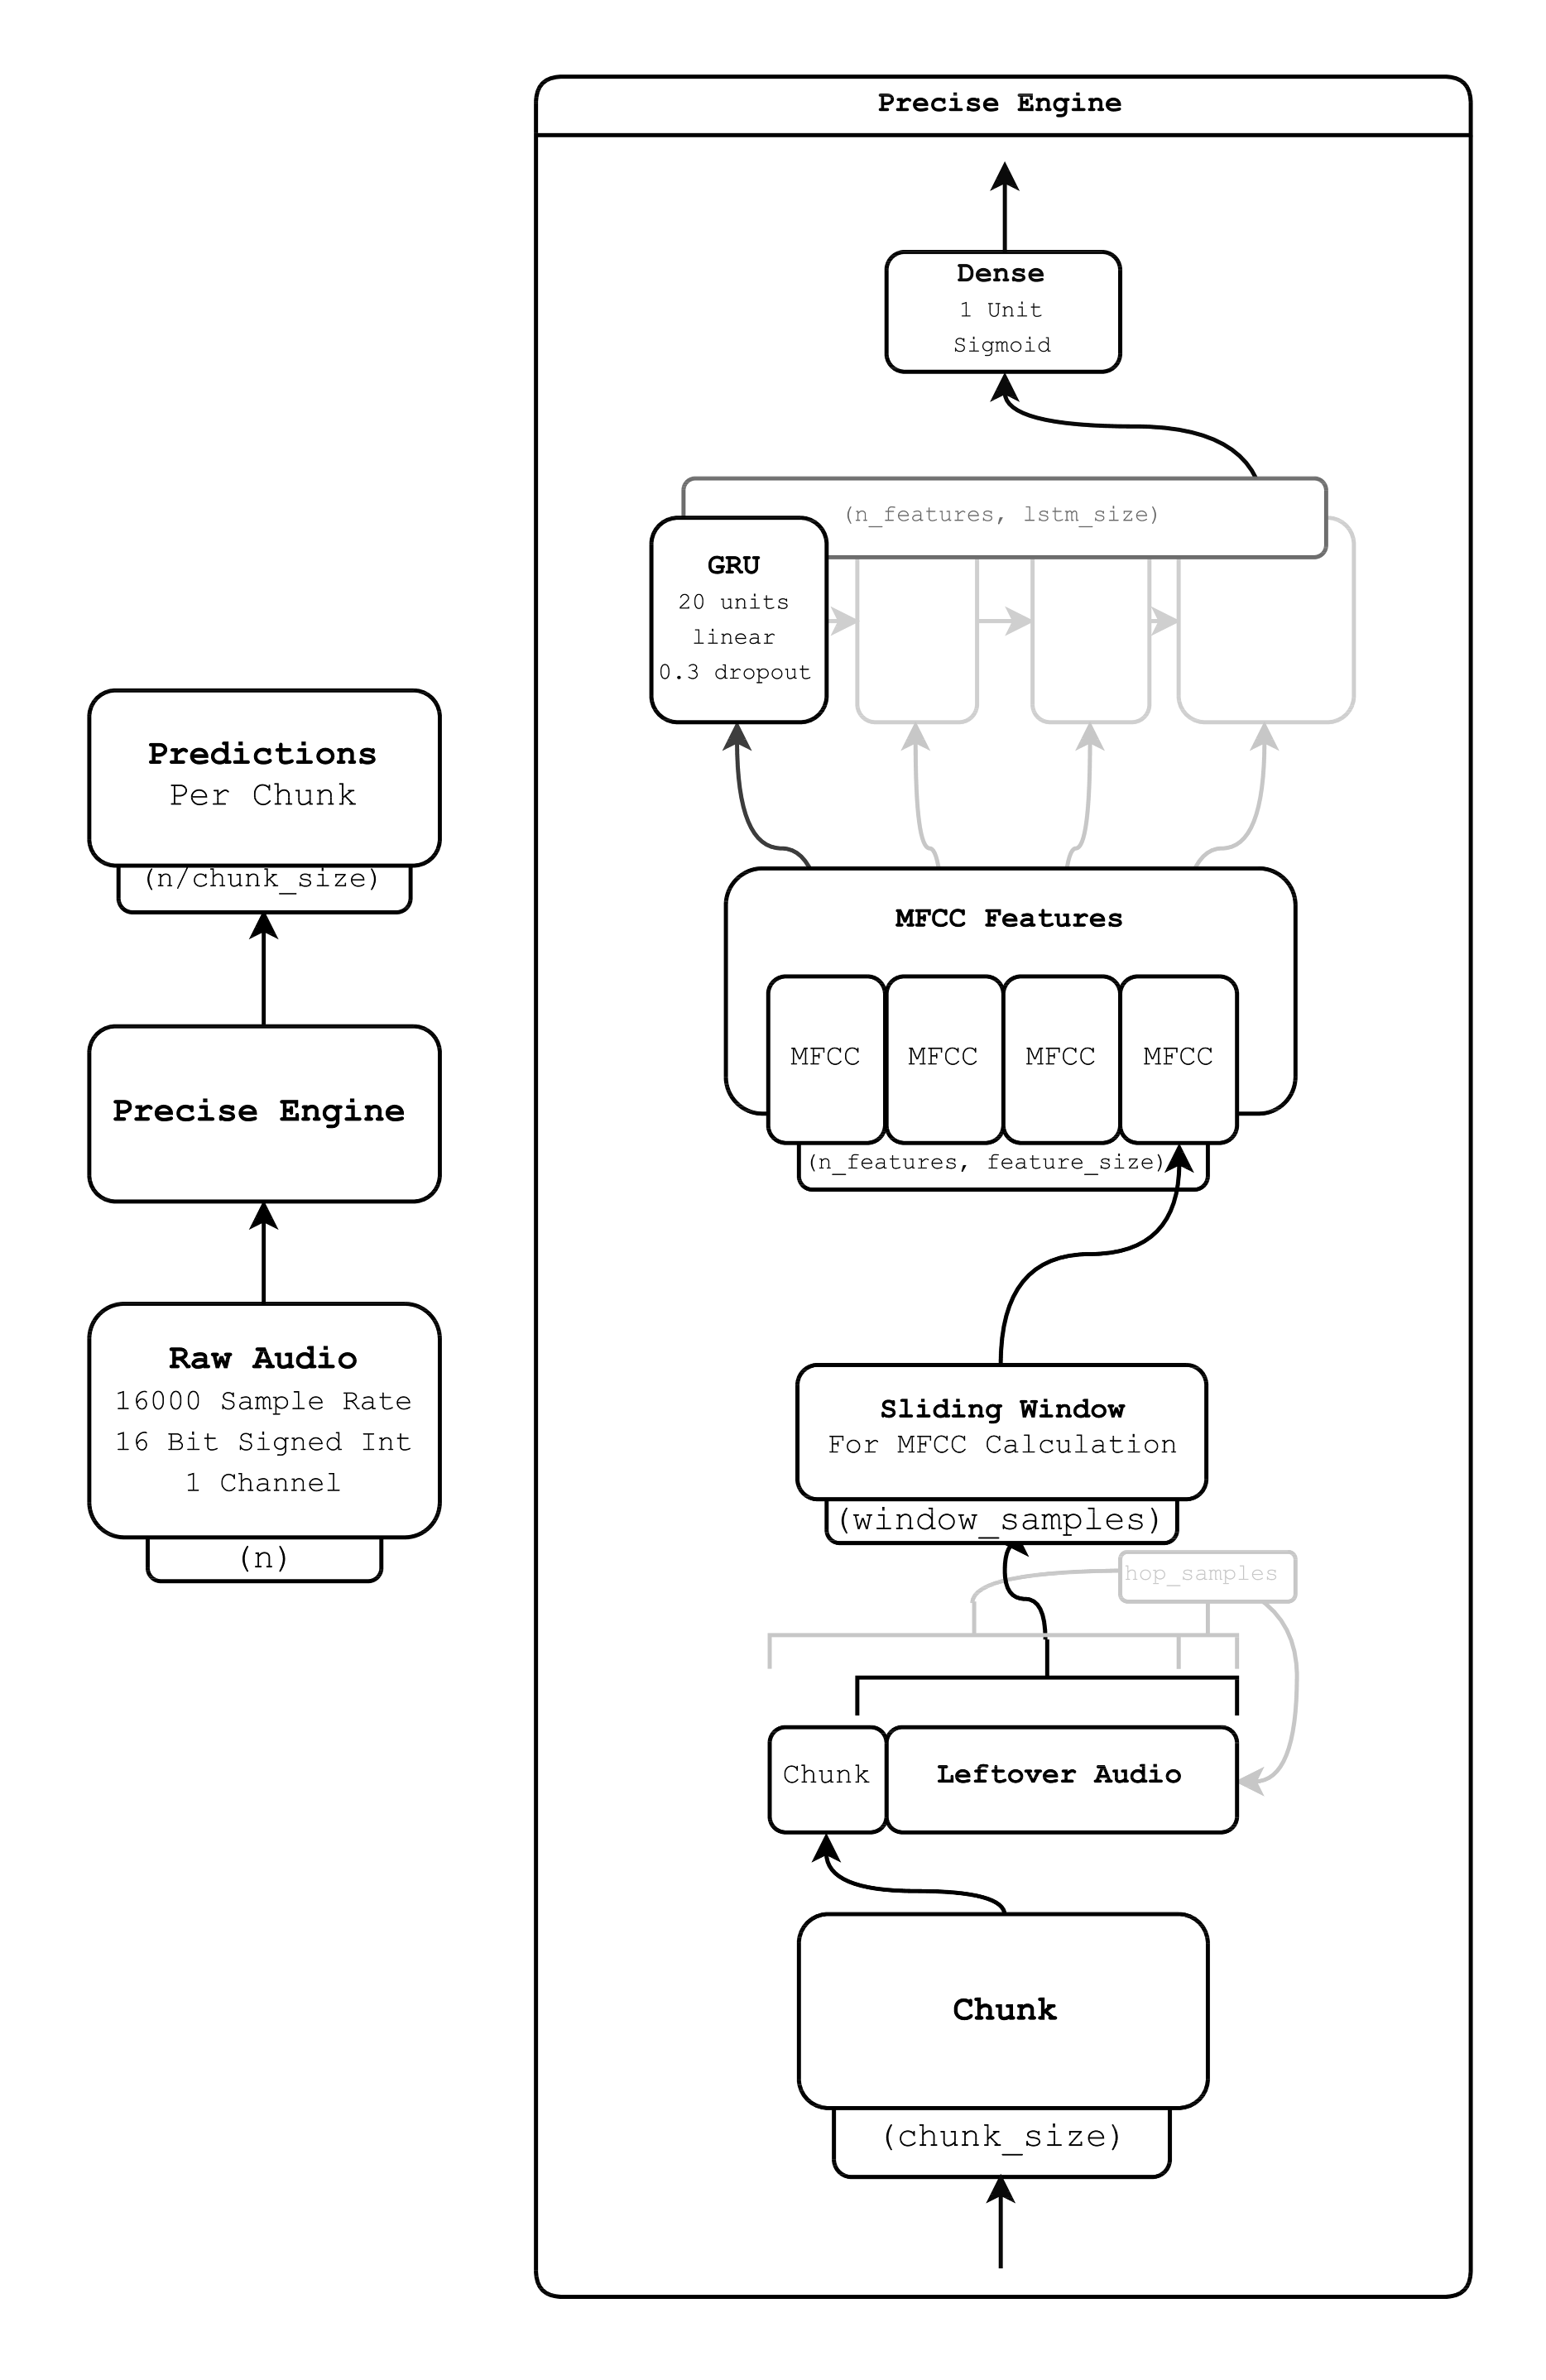
\includegraphics[width=0.6\columnwidth]{images/mycroft/precise.png}
    \end{center}
    \caption{Schema di funzionamento di Precise}
    \label{fig:precise}
\end{figure}
\subsubsection{Speech To Text}
Mycroft sfrutta il motore STT di Google per effettuare questo processo. Per aggiungere uno strato di privacy a queste richieste, esse vengono fatte passare attraverso i server Mycroft: Google non può ricollegare una richiesta all'utente che l'ha fatta. In questo modo, tutte le query effettuate a Google contengono solamente l'audio e hanno lo stesso mittente. In futuro sarà possibile sfruttare il dataset di \textbf{Mozilla Deepspeech}, che non è, ad oggi, ancora sufficientemente affidabile.
\subsubsection{Interpretazione degli intent}
Nell'ambito della speech recognition, un intent è l'operazione che l'utente \textit{intende} svolgere. Un utente può richiedere un'operazione in modi molto diversi. Lo scopo dell'intent parser è proprio quello di riuscire a superare questo scoglio, estraendo dalla richiesta scritta gli elementi chiave. Per esempio, se avessimo una richiesta del tipo "Hey Mycroft, domani pioverà a Parma?", l'intent parser dovrebbe capire:
\begin{itemize}
    \item L'utente desidera conoscere il \textbf{tempo atmosferico}
    \item Il tempo atmosferico deve essere cercato per \textbf{Parma}
    \item La data di interesse è \textbf{domani}
\end{itemize}
Mycroft rende disponibili due software per la rilevazione di intenti: Padatious e Adapt. Mentre il secondo è basato sul riconoscimento di parole chiave, ed è quindi molto suscettibile alle richieste, il primo è composto da una rete neurale addestrata su frasi intere. Nel corso del progetto sfrutteremo \textbf{Padatious}.
Questo motore permette di avere creazione semplice degli intent, quantità di dati relativamente bassa, estrazione delle \textit{entities} semplice, addestramento rapido.
\subsubsection{Text To Speech}
Il componente di Text To Speech ha il compito di generare una traccia audio partendo dal testo di risposta codificato nella skill. Mycroft rende disponibile il progetto \textbf{Mimic}, basato sul software FLITE dell'università Carnegie Mellon. Purtroppo quest'ultimo non è disponibile in italiano, quindi nel corso del progetto utilizzeremo il motore TTS di Google, ottimizzato per l'italiano. Come sempre, le richieste passano attraverso i server Mycroft per ottenere un buon livello di privacy.
I testi di risposta sono codificati nei file vocabolario delle skills.
\subsection{Interfaccia grafica}
I dispositivi più avanzati di Mycroft come il \textit{Mark II} forniscono la possibilità di aggiungere interazioni visive con gli utenti. L'interfaccia è gestita da Mycroft-GUI, un componente aggiuntivo del bot che sfrutta i KDE Plasmoids, oggetti dell'interfaccia grafica KDE Plasma, simili a widget. La tecnologia è basata sul linguaggio QML, che permette una totale libertà nella creazione di interfacce, ma anche dei template standard semplici e rapidi da implementare. QML fa parte dello stack di tecnologie di Qt, una libreria multipiattaforma per lo sviluppo di programmi con interfaccia grafica.